\pagebreak
\subsection{Solar cells in the dark}
So far, all the simulations we have run have been performed in the light.  This is a logical, as usually we are interested in solar cell performance only in the light.  However, a lot of interesting information can be gained about solar cells by studying their performance in the dark.  We are now going to turn off the light in the simulation.  From the \emph{Optical} tab set the \emph{Light intensity (suns)} drop down menu to 0.0 Suns, this can be seen in figure \ref{fig:dark}.  The photons in the 3D image should disappear as seen in figure \ref{fig:dark}.
\\
\\
\begin{minipage}{0.45\textwidth}
\centering
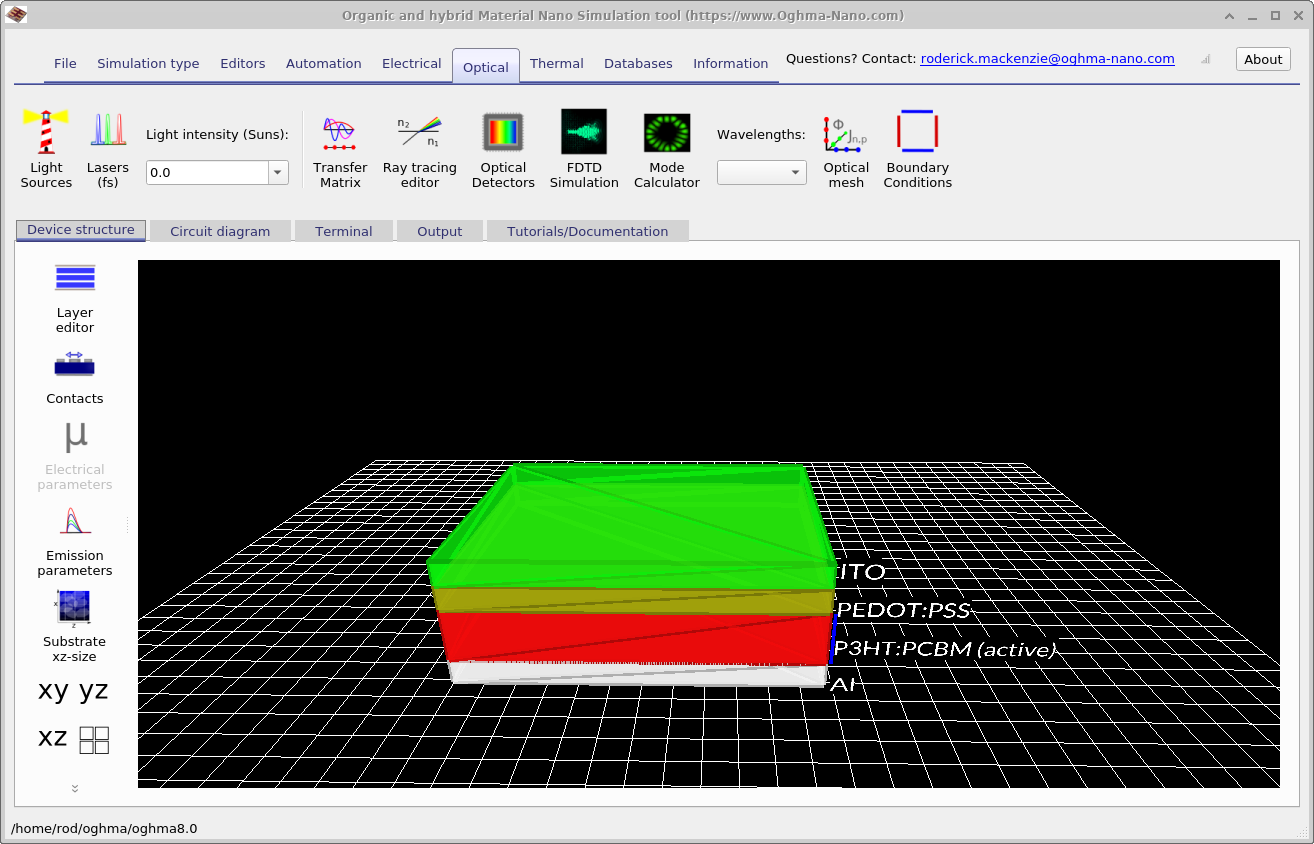
\includegraphics[width=\textwidth,height=0.7\textwidth]{./images/running/dark.png}
\captionof{figure}{Running OghmaNano in the dark, the Light intensity drop-down menu has been set to 0 Suns and the photons have disappeared from the image.}
\label{fig:dark}
\end{minipage}
\hspace*{10px}
\begin{minipage}[]{0.45\linewidth}
\centering
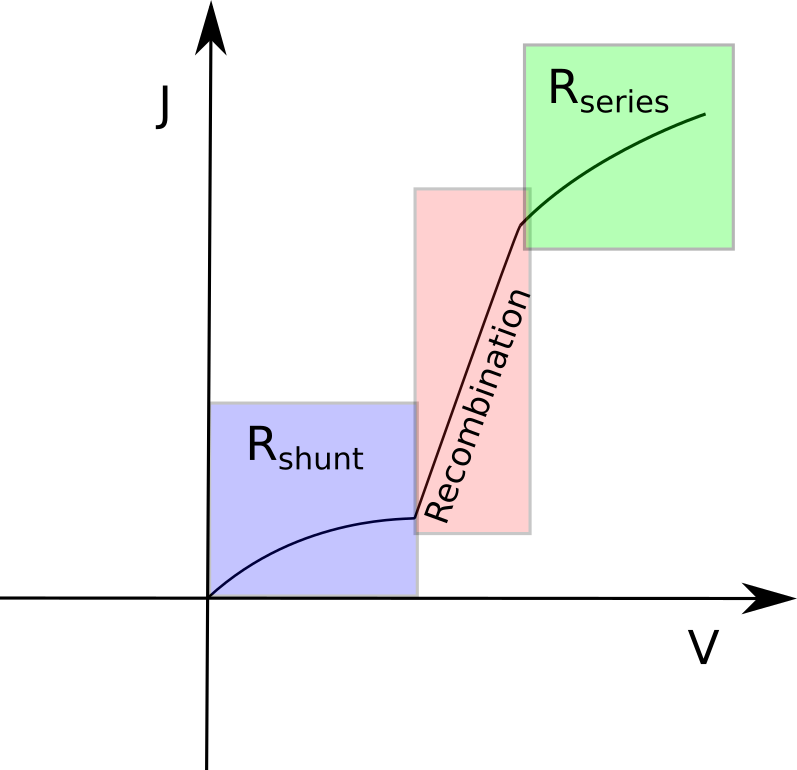
\includegraphics[width=\textwidth,height=0.7\textwidth]{./images/running/jv_dark.png}
\captionof{figure}{A sketch of a typical dark JV curve.}
\label{fig:jv_dark}
\end{minipage}
\\
\\
Now set the shunt resistance to $1M \Omega m^2$, and run a simulation.  Plot the jv curve.  It is customary to plot jv curves on a x-linear y-log scale.  To do this in the plot window, hit the 'l' key to do this.  The shape should resemble, the JV curve in figure \ref{fig:jv_dark}.  Certain solar cell parameters affect different parts of the dark JV curve differently, the lower region is affected very strongly by shunt resistance, the middle part is affected strongly by recombination, and the upper part is strongly affected by the series resistance.

\vspace*{\fill}
\fbox{
\parbox{0.9\textwidth}{
\color{blue} Question \addtocounter{question}{1}\thequestion: What values of series and shunt resistance, would produce the best possible solar cell?  Enter these values into the device simulator and copy and paste the dark JV curve into your report.
}\par
}


